\section{PI Measure}


\subsection{Formulation}

\begin{frame}{Formulation}

    The sets used to generate fields, and their correspondence to redundancy measures are defined as follows.
    \begin{block}{Basic Sets Correspondence}
        Denote the source variables domain as
        \begin{equation}
            \Gamma =  \left\{ \beta \in \mathcal{P}_{1}(\mathbf{R}) : \forall \mathbf{A}_i,\mathbf{A}_j \in \beta, \mathbf{A}_i \nsubseteq \mathbf{A}_j \right\}
        \end{equation}
        For every random variable collection in the domain $\Gamma$, its self-redundancy is defined as $I_{\min}\left(S;\left\{A_i, \ldots, A_j\right\}\right)$. We use $\left\{ \tilde{A}_{i}, \ldots, \tilde{A}_{j} \right\}$, or abbreviation $\tilde{A}_{i\ldots j}$ to represent the basic set its self redundancy corresponds to.
    \end{block}
\end{frame}

\begin{frame}{Formulation}
    To build fields, define the correspondence rules for operations on basic sets.
    \begin{block}{Field Correspondence}
        \begin{itemize}
            \item For every basic sets $\tilde{A}_{i\ldots j}$,
            \begin{equation}
                \mu^{*} \left(\tilde{A}_{i\ldots j}\right) = I_{\min}\left(S;\left\{A_i, \ldots, A_j\right\}\right).
                \label{eqn:intersectofbasic}
            \end{equation}
            \item For any two sets $\alpha$in the field, $\mu^{*} \left(\alpha^{c} \right) = \sum_{ \alpha \prec \gamma  } \Pi_{\mathbf{R}} (S;\gamma)$
            \item For any two sets $\alpha$ and $\beta$ in the field, $\mu^{*} \left(\alpha \cap \beta \right) = \sum_{\gamma \preceq \alpha \text{ and } \gamma \preceq \beta} \Pi_{\mathbf{R}} (S;\gamma)$
            \item For any two sets $\alpha$ and $\beta$, $\mu^{*} \left(\alpha \cup \beta \right) = \sum_{\gamma \preceq \alpha \text{ or } \gamma \preceq \beta} \Pi_{\mathbf{R}} (S;\gamma)$
            \item For any two sets $\alpha$ and $\beta$, $\mu^{*} \left(\alpha - \beta \right) = \sum_{\gamma \preceq \alpha \text{ and } \beta \prec \gamma} \Pi_{\mathbf{R}} (S;\gamma)$
        \end{itemize}
    \end{block}
    
    This definition is based on the partial order given in the redundancy lattice. However, such definition is not very useful in practice.
\end{frame}






\subsection{Simplification}
\begin{frame}{Simplification}
    We try to eliminate redundant fields in order to avoid the exponential increase of fields.
    
    \begin{block}{Example of Two Source Variables}
        To fix ideas, we take the multivariate information of three variables $I(S;\mathbf{A}_1, \mathbf{A}_2)$ as example, note that $\left\{ \tilde{A}_1 \right\} \subseteq \left\{\tilde{A}_1, \tilde{A}_2 \right\}$. It follows that 
        \begin{equation}
        \begin{aligned}
            \mu^{*}\left( \left\{ \tilde{A}_1 \right\} \cap \left\{\tilde{A}_1, \tilde{A}_2 \right\}^{C} \right) &= \mu^{*}\left( \left\{\tilde{A}_1\right\}\right)  - \mu^{*}\left(\left\{\tilde{A}_1 \right\}\cap  \left\{  \tilde{A}_1, \tilde{A_2} \right \} \right) \\
            &= I_{\min} \left( S; \left\{\mathbf{A}_1 \right\} \right) - I_{\min} \left( S; \left\{ \mathbf{A}_1 \right\} ,\left\{ \mathbf{A}_1, \mathbf{A}_2 \right\} \right) = 0
        \end{aligned}
        \label{eqn:fieldelim}
        \end{equation}
        Similarly, with the observation that $\left\{ \tilde{A}_2 \right\} \subseteq \left\{\tilde{A}_1, \tilde{A}_2 \right\}$, we have $\mu^{*}\left( \left\{ \tilde{A}_2 \right\} \cap \left\{\tilde{A}_1, \tilde{A}_2 \right\}^{C} \right) = 0$. To make our diagram more legible, we can erase these regions out.
    \end{block}
\end{frame}
    
\begin{frame}{Simplification}
    \begin{theorem}[Field Elimination] For any two basic sets $\tilde{A}_{i\ldots j} , \tilde{A}_{i' \ldots j'} \in \Gamma$, if $\tilde{A}_{i\ldots j} \subseteq \tilde{A}_{i' \ldots j'}$, then the measure of any set intersection with $\tilde{A}_{i\ldots j} \cap \tilde{A}_{i' \ldots j'}^{C}$ is zero.
    \end{theorem}
    
    
    \begin{figure}
        \centering
        \subfigure[$\tilde{A}_3$ produces no extra redundant fields]{
        \begin{minipage}[t]{0.3\linewidth}
        \centering
        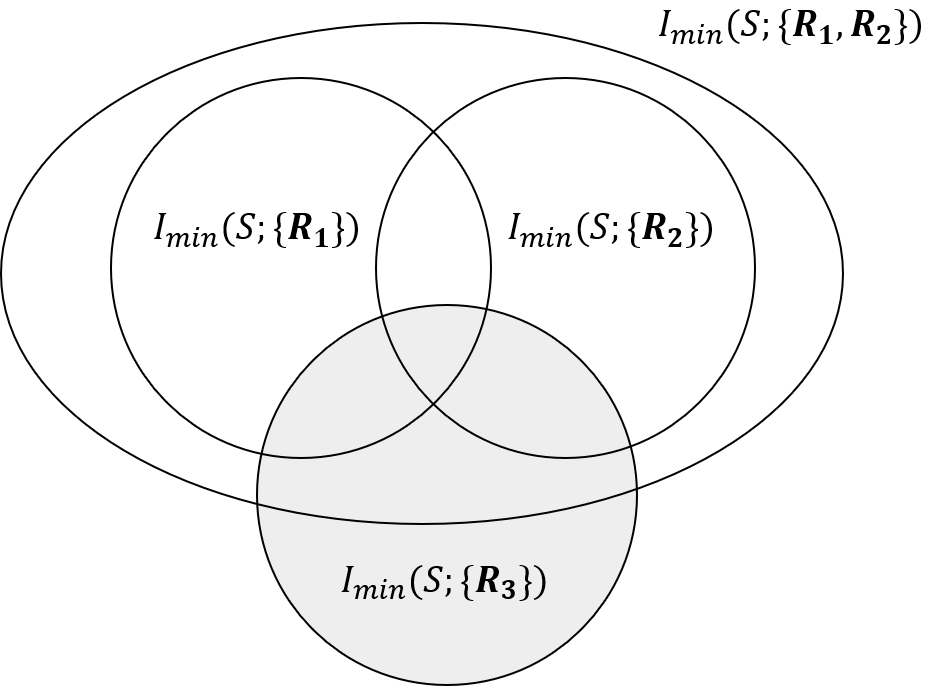
\includegraphics[height=2cm]{img/decompose1.png}
        %\caption{fig1}
        \end{minipage}%
        }%
        \quad
        \subfigure[Adding Basic Set $\tilde{A}_{12}$ produces extra redundant fields as has been starred]{
        \begin{minipage}[t]{0.3\linewidth}
        \centering
        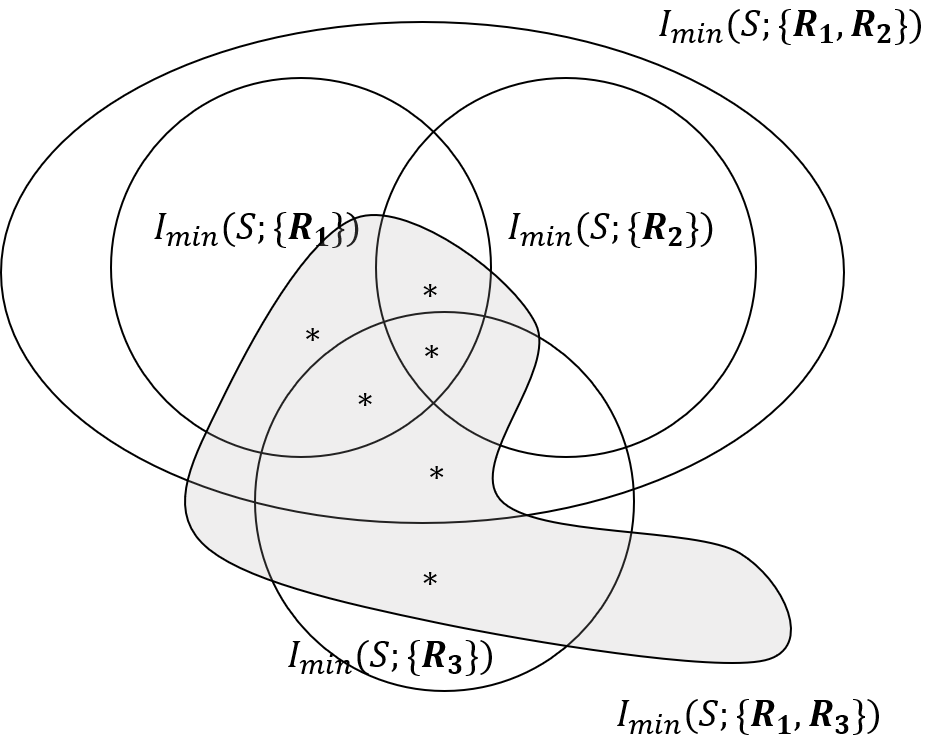
\includegraphics[height=2cm]{img/decompose2.png}
        %\caption{fig2}
        \end{minipage}%
        }%
        \quad
        \subfigure[After Elimination]{
        \begin{minipage}[t]{0.3\linewidth}
        \centering
        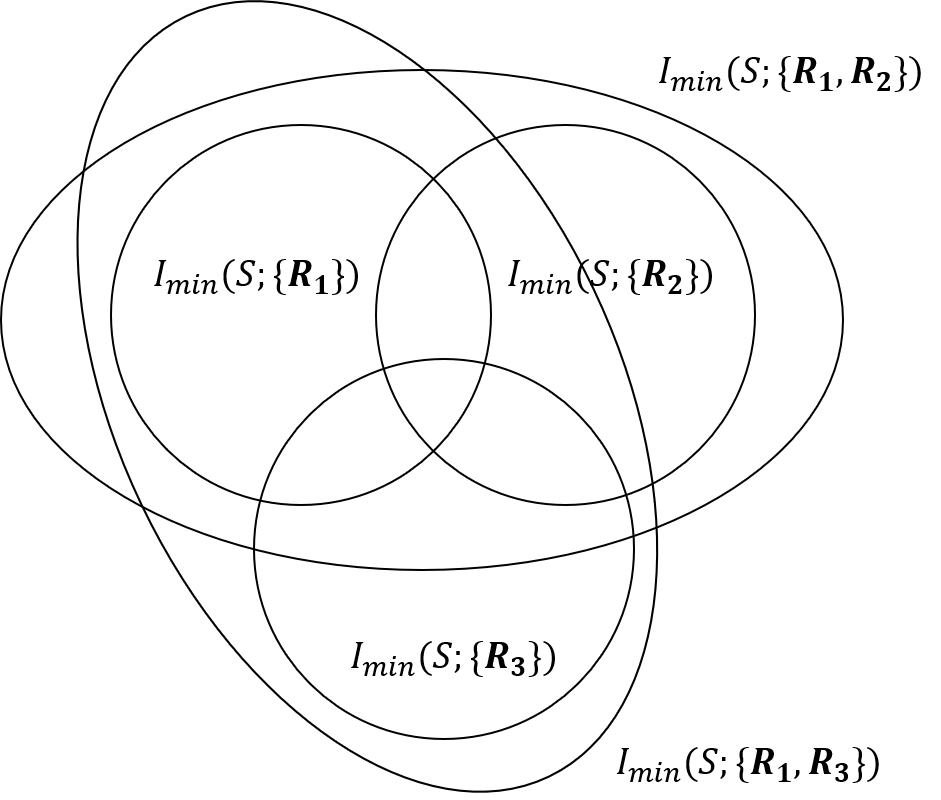
\includegraphics[height=2cm]{img/decompose3.png}
        %\caption{fig2}
        \end{minipage}%
        }%
        \centering
        \caption{Field Elimination Example for 3 Source Variables}
        \label{fig:elim4}
    \end{figure}
\end{frame}

\begin{frame}{Simplification}
    We try to find alternative, useful expressions of fields by means of set theory.
    \begin{block}{Observation on Atoms}
        \begin{itemize}
            \item  The measure of \textit{atoms} in $\mathcal{F}_n$ is a perfect matching to the partial information $\Pi_{\mathbf{R}}$.
            \item All redundancy measures can be written as sum of non-negative $\Pi_{\mathbf{R}}$s.
            \item All atoms can be written as sets of $\cap _{i\in\mathcal{N}_n} \tilde{Y}_i (\tilde{Y}_i = \tilde{A}_i \text{ or } \tilde{A}_i^c),$ where the index set $\mathcal{N}_n = \mathcal{P}_1\left(\left\{ 1,2,\ldots,n\right\}\right) $
        \end{itemize}
    \end{block}
    In order to completely write measure expressions, we only need to study two operations (complement and intersection) on basic sets $Y_{i \in \mathcal{N}_n}$.
\end{frame}

\begin{frame}{Simplification}
    \begin{align}
    & \mu^{*}\left( \tilde{A}_{N_1} \cap \ldots \cap \tilde{A}_{N_k} \cap \tilde{A}_{M_1}^{C} \cap \ldots\cap \tilde{A}_{M_j}^{C} \right) \\
    &= \mu^{*}\left(\tilde{A}_{N_1} \cap \ldots \cap \tilde{A}_{N_k} \right) - \sum_{i=1}^{k} \mu^{*} \left( \tilde{A}_{N_1} \cap \ldots \cap \tilde{A}_{N_k} \cap\tilde{A}_{M_1} \cap \ldots \cap \tilde{A}_{M_i} \right) \label{eqn:simplify}
    \end{align}

Note that in Equation \ref{eqn:simplify}, all the sets being measured are intersections of basic sets. By applying Equation \ref{eqn:intersectofbasic}, we can write them out in the form of redundancy measure $I_{\min}$.

\begin{block}{Conclusion}
\begin{itemize}
    \item The measure of any atom can be written as a $\pm 1$ combination of some redundancy measures $I_{\min}$.
    \item The measure of any field can be written as a linear combination of redundancy measures $I_{\min}$.
\end{itemize}
\end{block}
\end{frame}

\subsection{Application}
\begin{frame}{Application}
An application of our simplification is to calculate partial information in two ways. \\
\begin{block}{Method 1}
        On the one hand, we can using the definition of $\Pi_{\mathrm{R}}$ to calculate, applying Eq.\ref{ee1}.
\begin{equation}\Pi_{\mathbf{R}}(S ; \alpha)=I_{\min }(S ; \alpha)-\sum_{s} p(s) \max _{\beta \in \alpha^{-}} \min _{\mathbf{B} \in \beta} I(S=s ; \mathbf{B})
\label{ee1}
\end{equation}
    \end{block}
\begin{block}{Method 2}  
On the other hand, we can calculate $\Pi_{\mathrm{R}}$ by converting it to the linear combination of $I_{\min}$. 
\end{block}
\end{frame}

\begin{frame}{Example with Four Variables}
\begin{block}{Example}

 Consider three equiprobable cases of S as follows:
\[
\begin{array}{c}
\mathbf{S}=0: (\mathbf{R}_1=0,\mathbf{R}_2=0,\mathbf{R}_3=0)\\
\mathbf{S}=1: (\mathbf{R}_1=0,\mathbf{R}_2=1,\mathbf{R}_3=1)\\
\mathbf{S}=2: (\mathbf{R}_1=1,\mathbf{R}_2=0,\mathbf{R}_3=0)\\
\end{array}
\]
We want to calculate the value of $\Pi_{\mathrm{R}}(S ; \{2\},\{13\})$.
\end{block}

\end{frame}
\begin{frame}{Example with Four Variables}
\begin{block}{Method 1}Firstly, we can applying Eq.\ref{ee1}  to solve the problem:
\begin{equation}\Pi_{\mathbf{R}}(S ;\{2\},\{13\})=I_{\min }(S ; \{2\},\{13\})-\sum_{s} p(s) \max _{\beta \in \alpha^{-}} \min _{\mathbf{B} \in \beta} I(S=s ; \mathbf{B})\label{43}\end{equation} 
where $\beta \in\{\{\{1\}\{2\}\},\{\{2\}\{3\}\}\} $ . 
 Then we just need to expand the formula to calculate. We have
\begin{equation}I_{\min }(S ; \{2\},\{13\})=\log3 -\frac{2}{3} \log 2\end{equation}
\begin{equation}\sum_{s} p(s) \max _{\beta \in \alpha^{-}} \min _{\mathbf{B} \in \beta} I(S=s ; \mathbf{B})=\log3 -\frac{2}{3} \log 2\end{equation}
So $\Pi_{\mathrm{R}}(S ; \{2\},\{13\})$=0.
\end{block}


\end{frame}
\begin{frame}{Example with Four Variables}

\begin{block}{Method 2}
 based on the observations in FIG.\ref{fig:pi4}, we can express the field using Eq.\ref{eqn:intersectofbasic2}:
\begin{equation}
    \mu^{*}\left(\tilde{A}_{i \ldots j} \cap \ldots \cap \tilde{A}_{m \ldots n} \right) = I_{\min}\left(S; \left\{\mathbf{A}_i,\ldots,\mathbf{A}_j \right\}, \ldots,  \left\{\mathbf{A}_m,\ldots,\mathbf{A}_n \right\}\right)
    \label{eqn:intersectofbasic2}
\end{equation}

\[
\begin{array}{l}
   \mu^{*}\left( \left\{ \tilde{R}_1 \right\}^{C} \cap \left\{ \tilde{R}_2 \right\}\cap \left\{ \tilde{R}_3 \right\}^{C} \cap \left\{\tilde{R}_{12} \right\}\cap \left\{\tilde{R}_{13} \right\}\cap \left\{\tilde{R}_{23} \right\}\cap \left\{\tilde{R}_{123} \right\} \right)  \\
   
    =I_{\min} \left( S; \left\{ 2 \right\} ,\left\{ 1, 2 \right\} ,\left\{ 1, 3 \right\},\left\{ 2, 3 \right\},\left\{ 1, 2, 3 \right\}\right)  \\
     \quad- I_{\min} \left( S; \left\{ 1 \right\} ,\left\{ 2 \right\} ,\left\{ 1, 2 \right\} ,\left\{ 1, 3 \right\},\left\{ 2, 3 \right\},\left\{ 1, 2, 3 \right\}\right) \\
    \quad - I_{\min} \left( S; \left\{ 2 \right\} ,\left\{ 3 \right\} ,\left\{ 1, 2 \right\} ,\left\{ 1, 3 \right\},\left\{ 2, 3 \right\},\left\{ 1, 2, 3 \right\}\right) \\
     \quad+I_{\min} \left( S; \left\{ 1 \right\} ,\left\{ 2 \right\} ,\left\{ 3 \right\} ,\left\{ 1, 2 \right\} ,\left\{ 1, 3 \right\},\left\{ 2, 3 \right\},\left\{ 1, 2, 3 \right\}\right)\\
    =I_{\min} \left( S; \left\{ 2 \right\} ,\left\{ 1, 3 \right\}\right)  - I_{\min} \left( S; \left\{ 1 \right\} ,\left\{ 2 \right\} \right) - I_{\min} \left( S; \left\{ 2 \right\} ,\left\{ 3 \right\} \right) \\
    \quad+I_{\min} \left( S; \left\{ 1 \right\} ,\left\{ 2 \right\} ,\left\{ 3 \right\} \right)
\end{array}
\]
\end{block}


\end{frame}
\begin{frame}{Example with Four Variables}

\begin{block}{Method 2}


We can also list all $I_{\min}$ of the sets which have the partial order relation with $\{\{2\},\{13\}\}$ to express $\Pi_{\mathbf{R}}$ using the linear combination of $I_{\min}$.:

\begin{equation}
\begin{aligned}
&I_{\min }(S;\left\{2\},\{13\}\right)=\Pi_{\mathbf{R}}(S ;\{2\},\{3\})+\Pi_{\mathbf{R}}(S ;\{1\},\{2\}) \\ &+\Pi_{\mathbf{R}}(S ;\{2\},\{13\})+I_{\min }(S;\left\{1\},\{2\},\{3\}\right)\label{44}
\end{aligned}\end{equation}

\begin{equation}I_{\min }(S;\left\{2\},\{3\}\right)=\Pi_{\mathbf{R}}(S ;\{2\},\{3\})+I_{\min }(S;\left\{1\},\{2\},\{3\}\right)\label{45}\end{equation}

\begin{equation}I_{\min }(S;\left\{1\},\{2\}\right)=\Pi_{\mathbf{R}}(S ;\{1\},\{2\})+I_{\min }(S;\left\{1\},\{2\},\{3\}\right)\label{46}\end{equation}

Combine Eq.\ref{44},\ref{45},\ref{46}, then we have the save result as before.

Calculating by the linear combination of $I_{\min}$, we can also have the same outcome of $\Pi_{\mathrm{R}}(S ; \{2\},\{13\})$.\\
\end{block}
\end{frame}